\section{Build \taoce}

%%%%%%%%%%%%%%%%%%%%%%%%%%%%%%%%%%%%%%%%%%%%%%%%%%%%%%%%%%%%%%%%%%%%%%%%%%%%%%%%
\subsection{Process overview}
\begin{frame}
\begin{columns}[T]
\begin{column}{.3\textwidth}
\tikzstyle{arrow} = [thick,->,>=stealth]
\begin{center}
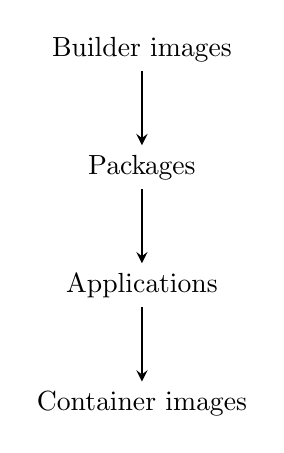
\begin{tikzpicture}[every text node part/.style={align=center},node distance=15mm]
    \node<1-> (base) {Builder images};
    \node<2-> (packages) [below of=base] {Packages};
    \node<3-> (apps) [below of=packages] {Applications};
    \node<4-> (images) [below of=apps] {Container images};

    \draw<2-> [arrow] (base) -- (packages);
    \draw<3-> [arrow] (packages) -- (apps);
    \draw<4-> [arrow] (apps) -- (images);
\end{tikzpicture}
\end{center}
\end{column}
\begin{column}{.7\textwidth}
    \begin{description}
        \item<1->[Builder images\notcovered] \taoce applications are built from PHP, NodeJS and Go builder images.
        \item<2->[Packages\notcovered] Some services depends from Composer and NPM packages, which will be built locally, and pushed to local registries (Verdaccio \& Satis).
        \item<3->[Applications] \taoce activities are separated in applications (Portal, Deliver, \dots).
        \item<4->[Container images\notcovered] Container images gather all the application artifacts and dependencies.
    \end{description}
\end{column}
\end{columns}
\end{frame}

%%%%%%%%%%%%%%%%%%%%%%%%%%%%%%%%%%%%%%%%%%%%%%%%%%%%%%%%%%%%%%%%%%%%%%%%%%%%%%%%
\subsection<article>{Builder images build process}
\begin{frame}<article>
    Builder images are built from their \href{https://github.com/tao-ce/tao-ce/blob/main/build/Taskfile.builds.yml}{\texttt{Taskfile.builds.yml}} file.

    \begin{description}
\item[build-base] supports building PHP and NodeJS applications.
\item[build.go] supports building Go applications.
    \end{description}

    They are kept in local \alert{Podman} registry (e.g \texttt{\scriptsize localhost/tao-ce/builds/base:dev-latest}).
\end{frame}

%%%%%%%%%%%%%%%%%%%%%%%%%%%%%%%%%%%%%%%%%%%%%%%%%%%%%%%%%%%%%%%%%%%%%%%%%%%%%%%%
\subsection<article>{Packages build process}
\begin{frame}<article>
    \taoce requires some packages to be built locally, and pushed to local registries (Verdaccio \& Satis).

    Those packages are built from \href{https://github.com/tao-ce/tao-ce/blob/main/packages/Taskfile.yml}{\texttt{Taskfile.yml}} and \href{https://github.com/tao-ce/tao-ce/blob/main/packages/Containerfile.in}{\texttt{Containerfile.in}} files.
\end{frame}

%%%%%%%%%%%%%%%%%%%%%%%%%%%%%%%%%%%%%%%%%%%%%%%%%%%%%%%%%%%%%%%%%%%%%%%%%%%%%%%%
\subsection{Applications build process}
\begin{frame}
    Each application is declared as a \href{https://github.com/tao-ce/tao-ce/blob/main/apps/Taskfile.yml\#L43-L58}{\texttt{Taskfile} namespace}. 

    E.g., building Deliver application will proceed as follows: 
    \begin{description}
    \item[:build] \begin{enumerate}
        \item \texttt{buildah} attempt to build \href{https://github.com/tao-ce/tao-ce/blob/main/apps/deliver/Containerfile.in\#L52-L64}{\texttt{export} target}.
        \item this target will require \texttt{build-backend} and \texttt{build-frontend} targets to be executed first.
        \item those targets will build their payloads from builder image.
    \end{enumerate}
    \item[:deploy] Application payload will be copied to \texttt{/opt/tao-ce/<application>} directory.
    \item[:start] Application \texttt{systemd} services will be started.
    \end{description}
\end{frame}

%%%%%%%%%%%%%%%%%%%%%%%%%%%%%%%%%%%%%%%%%%%%%%%%%%%%%%%%%%%%%%%%%%%%%%%%%%%%%%%%
\subsection<article>{Images build process}
\begin{frame}<article>
    Once all applications are ready, we can proceed with container image builds.

    \bigicon{\faCamera}

    \begin{enumerate}
        \item A dedicated Base image is built
        \item Depending on choosen \alert{flavor}, applications are added to the image in \texttt{/opt/tao-ce} directory
        \item The image is then pushed to the local registry
    \end{enumerate}
\end{frame}

%%%%%%%%%%%%%%%%%%%%%%%%%%%%%%%%%%%%%%%%%%%%%%%%%%%%%%%%%%%%%%%%%%%%%%%%%%%%%%%%
\subsection{Tasks}
\begin{frame}
    Main tasks:
    \begin{description}
        \item[dev:up] Build and start all \taoce services.
        \item[dev:setup] Refresh \taoce \devcontainer configuration.
        \item[swift:build] Build \taoce container image.
        \item[dev:down] Stop and remove \taoce services.
        \item[dev:prune] Remove all build resources.
    \end{description}

    \only<presentation>{More tasks\notcovered are defined by application namespace.}
\end{frame}

%%%%%%%%%%%%%%%%%%%%%%%%%%%%%%%%%%%%%%%%%%%%%%%%%%%%%%%%%%%%%%%%%%%%%%%%%%%%%%%%
\begin{frame}<article>
    Each application has also its own set of tasks (e.g. for Portal):
    \begin{description}
        \item[apps:portal:up] Build, deploy and start Portal services.
        \item[apps:portal:build] Build the Portal application.
        \item[apps:portal:deploy] Copy Portal application files in \texttt{/opt/tao-ce/portal}.
        \item[apps:portal:start] Start Portal services.
        \item[apps:portal:restart] Restart Portal services.
        \item[apps:portal:stop] Stop Portal services.
    \end{description}
\end{frame}

%%%%%%%%%%%%%%%%%%%%%%%%%%%%%%%%%%%%%%%%%%%%%%%%%%%%%%%%%%%%%%%%%%%%%%%%%%%%%%%%
\subsection{Logging \& Debug}
\begin{frame}[fragile=singleslide]
All building logs are forwarded to \texttt{JournalD}
\inputminted{bash}{./snippets/journalctl.sh}

\TAOCE services may access the following directories:
\begin{description}
    \item[\texttt{/opt/tao-ce}] Application runtime
    \item[\texttt{/etc/tao-ce/setup}] Generated applications configuration
    \item[\texttt{/var/lib/tao-ce}] Applications data and cache
\end{description}
\end{frame}